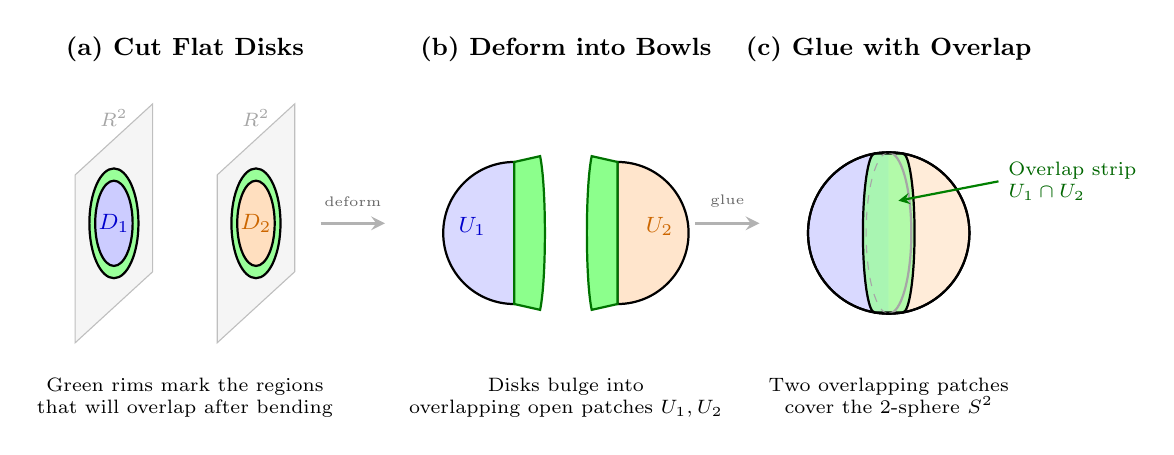
\begin{tikzpicture}[scale=0.82, >=stealth]
  % -------------------------------------------------------------
  % Panel 1: Cut two disks from parallel planes
  % -------------------------------------------------------------
  \begin{scope}[shift={(0,0)}]
    \node[above, font=\bfseries\small] at (1.3, 2.5) {(a) Cut Flat Disks};
    
    % Left plane
    \draw[gray!50, fill=gray!8] (-0.4, -1.7) -- (0.8, -0.6) -- (0.8, 2.0) -- (-0.4, 0.9) -- cycle;
    \node[above, gray!70, font=\scriptsize] at (0.2, 1.5) {$\mathbb{R}^2$};
    % Left disk with a green rim marking the future overlap collar
    \draw[thick, fill=green!40] (0.2, 0.15) ellipse (0.38 and 0.85);
    \draw[thick, fill=blue!20] (0.2, 0.15) ellipse (0.29 and 0.66);
    \node[font=\footnotesize, text=blue!80!black] at (0.2, 0.15) {$D_1$};
    \coordinate (chart-D1) at (0.55,0.15);

    % Right plane
    \draw[gray!50, fill=gray!8] (1.8, -1.7) -- (3.0, -0.6) -- (3.0, 2.0) -- (1.8, 0.9) -- cycle;
    \node[above, gray!70, font=\scriptsize] at (2.4, 1.5) {$\mathbb{R}^2$};
    % Right disk with a matching future overlap collar
    \draw[thick, fill=green!40] (2.4, 0.15) ellipse (0.38 and 0.85);
    \draw[thick, fill=orange!25] (2.4, 0.15) ellipse (0.29 and 0.66);
    \node[font=\footnotesize, text=orange!80!black] at (2.4, 0.15) {$D_2$};
    \coordinate (chart-D2) at (2.75,0.15);

    \node[below, font=\scriptsize, align=center] at (1.3, -2.1) {Green rims mark the regions\\that will overlap after bending};
  \end{scope}

  % Arrow 1 -> 2
  \draw[->, very thick, gray!60] (3.4, 0.15) -- (4.4, 0.15) node[midway, above=2pt, font=\tiny, text=gray!80!black] {deform};

  % -------------------------------------------------------------
  % Panel 2: Deform into overlapping open patches
  % -------------------------------------------------------------
  \begin{scope}[shift={(6.2,0)}]
    \node[above, font=\bfseries\small] at (1.0, 2.5) {(b) Deform into Bowls};

    % Surface strips match the patches in sphere_transition.tex.
    \draw[thick, fill=blue!15]
      (0.2, 1.1) arc (90:270:1.1 and 1.1) -- cycle;
    \path[fill=green!45, draw=green!45!black, thick]
      (0.2,1.1) -- (0.2,-1.1) -- (0.60,-1.19)
      .. controls (0.70,-0.73) and (0.70,0.73) .. (0.60,1.19) -- cycle;
    \node[font=\footnotesize, text=blue!80!black] at (-0.45, 0.1) {$U_1$};
    \coordinate (chart-U1) at (0.0,0.9);
    \coordinate (transition-U1) at (0.5,0.15);

    \draw[thick, fill=orange!20]
      (1.8, 1.1) arc (90:-90:1.1 and 1.1) -- cycle;
    \path[fill=green!45, draw=green!45!black, thick]
      (1.8,1.1) -- (1.8,-1.1) -- (1.40,-1.19)
      .. controls (1.30,-0.73) and (1.30,0.73) .. (1.40,1.19) -- cycle;
    \node[font=\footnotesize, text=orange!80!black] at (2.45, 0.1) {$U_2$};
    \coordinate (chart-U2) at (2.4,0.8);
    \coordinate (transition-U2) at (1.5,0.15);

    \node[below, font=\scriptsize, align=center] at (1.0, -2.1) {Disks bulge into\\overlapping open patches $U_1, U_2$};
  \end{scope}

  % Arrow 2 -> 3
  \draw[->, very thick, gray!60] (9.2, 0.15) -- (10.2, 0.15) node[midway, above=2pt, font=\tiny, text=gray!80!black] {glue};

  % -------------------------------------------------------------
  % Panel 3: Glued together with overlapping strip
  % -------------------------------------------------------------
  \begin{scope}[shift={(12.2,0)}]
    \node[above, font=\bfseries\small] at (0, 2.5) {(c) Glue with Overlap};

    % Left hemisphere (blue)
    \draw[thick, fill=blue!15] (0, 1.25) arc (90:270:1.25);
    
    % Right hemisphere (orange)
    \draw[thick, fill=orange!15] (0, 1.25) arc (90:-90:1.25);

    % Overlapping collar / strip in center (green tint)
    \draw[thick, fill=green!40, fill opacity=0.75] 
      (-0.22, 1.23) arc (90:270:0.18 and 1.23) 
      -- (0.22, -1.23) arc (-90:90:0.18 and 1.23) -- cycle;
      
    % Central boundary curve
    \draw[dashed, gray!70] (0, 1.25) arc (90:270:0.35 and 1.25);
    \draw[thick, gray!70] (0, 1.25) arc (90:-90:0.35 and 1.25);

    % Full sphere circle boundary
    \draw[thick] (0,0) circle (1.25);

    % Callout for overlap placed clearly outside the sphere to the right
    \draw[->, thick, green!50!black] (1.7, 0.8) -- (0.15, 0.5);
    \node[right, font=\scriptsize, align=left, text=green!40!black] at (1.7, 0.8) {Overlap strip\\$U_1 \cap U_2$};

    \node[below, font=\scriptsize, align=center] at (0, -2.1) {Two overlapping patches\\cover the 2-sphere $S^2$};
  \end{scope}

  % The chart-map slide enables these arrows; the original figure omits them.
  \ifdefined\showchartmaps
    \draw[->, very thick, blue!80!black]
      (chart-U1) .. controls +(-0.4,1.8) and +(0.8,2.4) .. (chart-D1)
      node[midway, above=4pt, font=\small] {$\phi_1$};
    \draw[->, very thick, orange!80!black,
        preaction={draw=white,line width=3.5pt}]
      (chart-U2) .. controls +(-1.0,1.9) and +(1.0,2.2) .. (chart-D2)
      node[midway, above=4pt, font=\small] {$\phi_2$};
  \fi

  % A separate variant traces one point through a coordinate transition.
  \ifdefined\showtransitionmaps
    \draw[->, very thick, blue!80!black, shorten <=3pt, shorten >=3pt]
      (chart-D1) .. controls +(0.9,2.2) and +(-0.2,2.2) .. (transition-U1)
      node[midway, above=4pt, font=\small] {$\phi_1^{-1}$};
    \draw[->, very thick, orange!80!black, shorten <=3pt, shorten >=3pt,
        preaction={draw=white,line width=3.5pt}]
      (transition-U2) .. controls +(-0.3,2.0) and +(1.0,2.4) .. (chart-D2)
      node[midway, above=4pt, font=\small] {$\phi_2$};
    \draw[densely dashed, thick, red!80!black, shorten <=4.5pt, shorten >=4.5pt]
      (transition-U1) -- (transition-U2);
    \draw[->, very thick, red!80!black, shorten <=3pt, shorten >=3pt]
      (chart-D1) .. controls +(0.3,-1.65) and +(0.6,-1.65) .. (chart-D2)
      node[midway, below=3pt, font=\small] {$\phi_2\circ\phi_1^{-1}$};
    \foreach \point in {chart-D1,transition-U1,transition-U2,chart-D2}
      \filldraw[fill=red!85!black,draw=white,line width=0.35pt]
        (\point) circle[radius=2.2pt];
    \node[below=10pt,font=\scriptsize,text=red!80!black] at (transition-U1) {$p$};
    \node[below=10pt,font=\scriptsize,text=red!80!black] at (transition-U2) {$p$};
  \fi
\end{tikzpicture}
